\documentclass[a4paper]{article}

%% Language and font encodings
\usepackage[english]{babel}
\usepackage[utf8x]{inputenc}
\usepackage[T1]{fontenc}

%% Sets page size and margins
\usepackage[a4paper,top=3cm,bottom=2cm,left=3cm,right=3cm,marginparwidth=1.75cm]{geometry}

%% Useful packages
\usepackage{amsmath}
\usepackage{graphicx}
\usepackage[colorinlistoftodos]{todonotes}
\usepackage[colorlinks=true, allcolors=blue]{hyperref}

\title{Cahier des charges\\ Plate-forme de calcul distribué en JavaScript}
%\title{Plate-forme de calcul javascript}
\author{Taoukilite Ahmed El Mahdi}

\begin{document}
\maketitle

\section{Présentation du projet}
\subsection{Contexte}
Le projet consiste a concevoir une plate-forme de calcul massive distribuée, basé sur la volontariat, et qui permettras au chercheurs d'avoir la puissance calculs de nombreux ordinateur personnels dans le monde entier. Les calculs seront effectué sur les machines volontaires et les résultats seront renvoyer a la plate-forme.

 


\subsection{Objectifs}
La plate-forme propose un service web avec deux interfaces web:
\begin{itemize}
\item Une interface administrateur (Figure \ref{fig:ProtoChercheur}): qui permet aux chercheurs d'écrire un code JavaScript du calcul, et de l'envoyer au serveur et exécuter ce code dans les machines volontaires.   
\item Une interface volontaire : qui permet la participation au calculs, en recevant des codes JavaScript a exécuter et de retourner les résultats au serveur web.
 Un volontaire est connecté sur la plate-forme quand il visite l'interface dédié aux volontaires, et se déconnecte quand il change ou ferme le site web. 
%\item Un service gestionnaire de files de messages, qui contiendras deux file par calcul, une file de jobs et une file de résultats

\end{itemize}


\section{Fonctionnement}

\subsection{Architecture de la plate-forme}
La plate-forme (Figure \ref{fig:ArchGenarale}) contient 3 serveurs et une base de donnée :
\begin{itemize}
\item Un serveur web (type NodeJS) pour gérer les volontaires, qui effectue les opérations suivantes:
\begin{itemize}
\item Récupération des jobs a partir de la file des jobs.
\item Envoie des jobs aux volontaires.
\item Récupération des résultats du job exécuter par le volontaire.
\item Dépôts des résultats dans la file des résultats
\end{itemize} 
\item Un serveur web (type NodeJS) pour gérer les chercheurs, qui effectue les opérations suivantes:
\begin{itemize}
\item Récupération le code JavaScript du calcul
\item Génération et dépôt des jobs à la file des jobs.
\item Récupération des résultats du calcul a partir la file des résultats.
\end{itemize} 

\end{itemize}  


\subsection{Annexe}
\begin{figure}
\centering
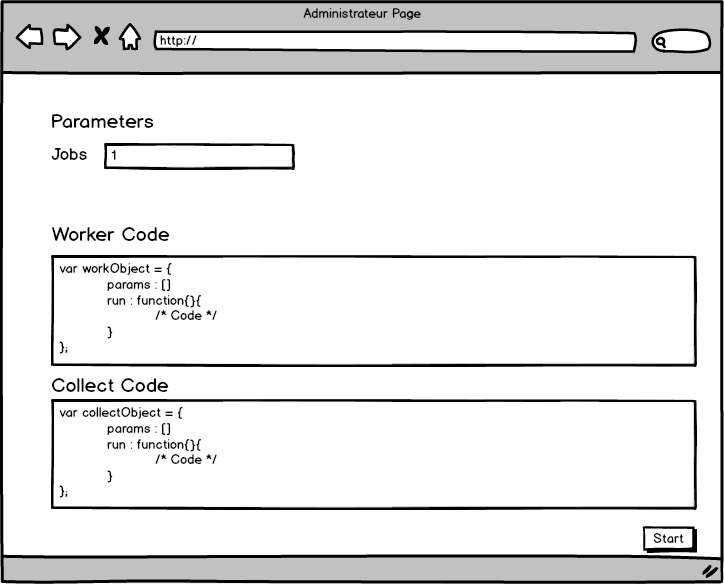
\includegraphics[width=0.7\textwidth]{calc1.png}
\caption{\label{fig:ProtoChercheur}Prototype Interface Chercheurs}
\end{figure}
\begin{figure}
\centering
\includegraphics[width=0.6\textwidth]{ArchGen.png}
\caption{\label{fig:ArchGenarale}Architecture générale de la plate-forme}
\end{figure}




\end{document}
